%% This Beamer template is based on the one found here: https://github.com/sanhacheong/stanford-beamer-presentation, and edited to be used for Stanford ARM Lab

\documentclass[10pt]{beamer}
%\mode<presentation>{}

\usepackage{media9}
\usepackage{amssymb,amsmath,amsthm,enumerate}
\usepackage[utf8]{inputenc}
\usepackage{array}
\usepackage[parfill]{parskip}
\usepackage{graphicx}
\usepackage{caption}
\usepackage{subcaption}
\usepackage{bm}
\usepackage{amsfonts,amscd}
\usepackage[]{units}
\usepackage{listings}
\usepackage{multicol}
\usepackage{multirow}
\usepackage{tcolorbox}
\usepackage[T2A]{fontenc} % enable Cyrillic fonts
\usepackage[utf8]{inputenc} % make weird characters work
\usepackage[serbianc]{babel}
% Enable colored hyperlinks
\hypersetup{colorlinks=true}

% Numbered captions of tables, pictures, etc.
\setbeamertemplate{caption}[numbered]


\newcommand{\empy}[1]{{\color{darkorange}\emph{#1}}}
\newcommand{\empr}[1]{{\color{cardinalred}\emph{#1}}}
\newcommand{\examplebox}[2]{
\begin{tcolorbox}[colframe=darkcardinal,colback=boxgray,title=#1]
#2
\end{tcolorbox}}

\DeclareMathOperator{\mex}{mex}
\DeclareMathOperator{\comma}{,}
\DeclareMathOperator{\equal}{=}
\DeclareMathOperator{\leftbracket}{[}
\DeclareMathOperator{\rightbracket}{]}
\usetheme{Stanford} 
%\def \i  {\item}
\def \ai {\item[] \quad \arrowbullet}
\newcommand \si[1]{\item[] \quad \bulletcolor{#1}}
\def \wi {\item[] \quad $\ \phantom{\Rightarrow}\ $}
\def \bi {\begin{itemize}\item}
\def \ei {\end{itemize}}
\def \be {\begin{equation*}}
\def \ee {\end{equation*}}
\def \bie {$\displaystyle{}
\def \eie {{\ }$}}
\def \bsie {\small$\displaystyle{}
\def \esie {{\ }$}\normalsize\selectfont}
\def \bse {\small\begin{equation*}}
\def \ese {\end{equation*}\normalsize}
\def \bfe {\footnotesize\begin{equation*}}
\def \efe {\end{equation*}\normalsize}
\renewcommand \le[1] {\\ \medskip \lefteqn{\hspace{1cm}#1} \medskip}
\def \bex {\begin{example}}
\def \eex {\end{example}}
\def \bfig {\begin{figure}}
\def \efig {\end{figure}}
\def \btheo {\begin{theorem}}
\def \etheo {\end{theorem}}
\def \bc {\begin{columns}}
\def \ec {\end{columns}}
\def \btab {\begin{tabbing}}
\def \etab {\end{tabbing}\svneg\svneg}
\newcommand \col[1]{\column{#1\linewidth}}
\def\vneg  {\vspace{-5mm}}
\def\lvneg {\vspace{-10mm}}
\def\svneg {\vspace{-2mm}}
\def\tvneg {\vspace{-1mm}}
\def\vpos  {\vspace{5mm}}
\def\lvpos {\vspace{10mm}}
\def\svpos {\vspace{2mm}}
\def\tvpos {\vspace{1mm}}
\def\hneg  {\hspace{-5mm}}
\def\lhneg {\hspace{-10mm}}
\def\shneg {\hspace{-2mm}}
\def\thneg {\hspace{-1mm}}
\def\hpos  {\hspace{5mm}}
\def\lhpos {\hspace{10mm}}
\def\shpos {\hspace{2mm}}

\logo{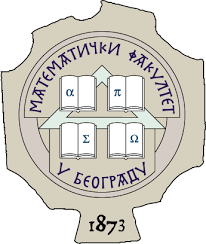
\includegraphics[height=0.4in]{./matf_logo.png}}

% commands to relax beamer and subfig conflicts
% see here: https://tex.stackexchange.com/questions/426088/texlive-pretest-2018-beamer-and-subfig-collide
%\makeatletter
%\let\@@magyar@captionfix\relax
%\makeatother

\title[Игра ним]{
	{\huge Игра ним}
}
%\subtitle{Subtitle Of Presentation}

\beamertemplatenavigationsymbolsempty
%\vspace{10ex}
\begin{document}
\author[Марија Мијаиловић]{	
	%\vspace{-5ex}
	{
		\parbox{0.45\textwidth}
			{\raggedright \textit{Аутор}:\\Марија Мијаиловић}
			\hfill
		\parbox{0.45\textwidth}
		{\raggedleft \textit{Ментор}:\\проф.др Миодраг Живковић}
	}
}

\institute{
	\begin{figure}
		\centering
		\begin{subfigure}[t]{0.5\textwidth}
			\centering
			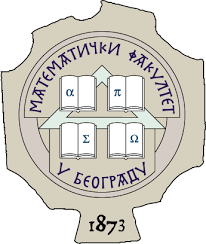
\includegraphics[height=0.33in]{./matf_logo.png}
		\end{subfigure}%
	\end{figure}
	{\footnotesize{Математички факултет}}\\
	{\footnotesize{Универзитет у Београду}}
}

\date{{\scriptsize{Септембар, 2020}}}

\begin{noheadline}
\begin{frame}\maketitle\end{frame}
\end{noheadline}

\setbeamertemplate{itemize items}[default]
\setbeamertemplate{itemize subitem}[circle]

\begin{frame}
	\frametitle{Садржај} % Table of contents slide, comment this block out to remove it
	\tableofcontents % Throughout your presentation, if you choose to use \section{} and \subsection{} commands, these will automatically be printed on this slide as an overview of your presentation
\end{frame}

\section{Игра ним}
% `[allowframebreaks]` can be used to have multiple slides in one frame, where the slides are continued with the suffix "(cont.)"; `[allowframebreaks]` can be used with `\framebreak` to manually break each frame into multiple slides

	\begin{frame}{Игра ним}
		\begin{itemize}
			\item Два играча
			\item Број жетона и гомила на столу одређују сами играчи
			\item Жетони се узимају само са једне гомиле, и мора се узети бар један жетон
			\item Нормални и мизерни ним
		\end{itemize}
	\end{frame}		
%
%	\begin{frame}{Варијантe нима}
%		\begin{itemize}
%			\item Нормални ним
%			\item Мизерни ним
%			\item Индекс k игра
%			\item Похлепни ним
%			\item Градитељски ним
%			\item Витховофа игра
%		\end{itemize}
%	\end{frame}
		
	\begin{frame}{Пример партије нормалног нима}
		\begin{figure}
	        \centering
	        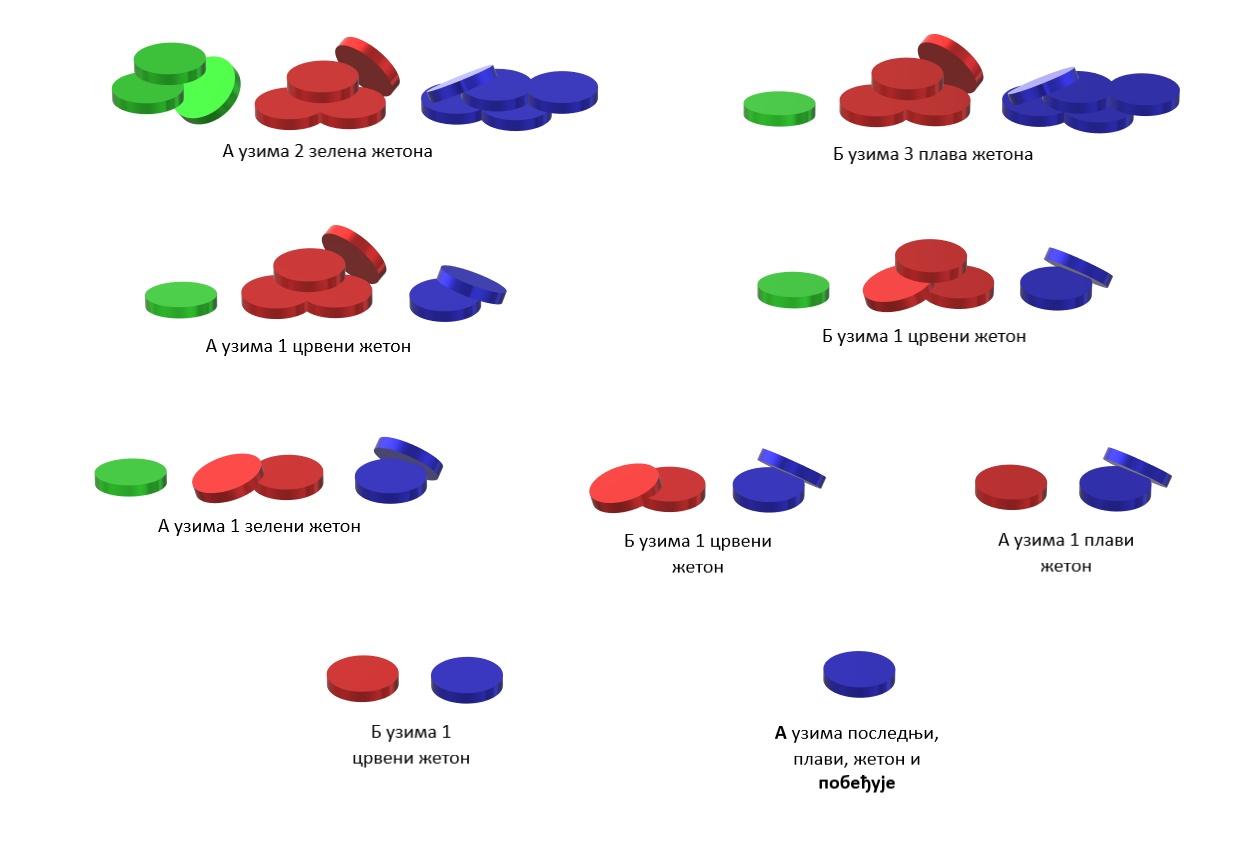
\includegraphics[width=0.8\textwidth]{../src/statistics/picture/NimPrimer.png}
	    \end{figure}
	\end{frame}

\section{Витхофова игра}
	\begin{frame}{Шта је Витхофова игра?}
		
		\begin{itemize}
			\item Две гомиле жетона
			\item Жетони се узимају са једне или обе гомиле
			\item Све позиције се могу разврстати у добитне и изгубљене
		\end{itemize}
	\end{frame}

%	\begin{frame}{Оптимална стратегија за Витхофову игру}
%		Да би се Витхофова игра играла на најбољи могући начин, потребно је знати две ствари:
%		\begin{itemize}
%			\item Препознати природу тренутне позиције, да ли је добитна или изгубљена.
%			\item Уколико је тренутна позиција добитна, треба одредити следећи потез тако да се противник нађе у изгубљеној позицији.
%		\end{itemize}		
%	\end{frame}
	
	\begin{frame}{Изгубљене позиције за $ a = 1 $}
		\begin{center}
			\begin{minipage}[t]{.20\linewidth}
				\begin{table}[h!]
					\begin{center}
						\begin{tabular}{  c | c | c }
							{\textbf{n}} &  {\textbf{A}} &  {\textbf{B}} \\
							\hline
							0 & 0 & 0 \\
							1 & 1 & 2 \\
							2 & 3 & 5 \\
							3 & 4 & 7 \\
							4 & 6 & 10 \\
							5 & 8 & 13 \\
							6 & 9 & 15 \\
							7 & 11 & 18 \\
							8 & 12 & 20 \\
							9 & 14 & 23 \\
							10 & 16 & 26\\
							11 & 17 & 28\\ 
						\end{tabular}
					\end{center}
				\end{table}
			\end{minipage}%
			\begin{minipage}[t]{.80\linewidth}
				\vspace{0pt}
				\centering
				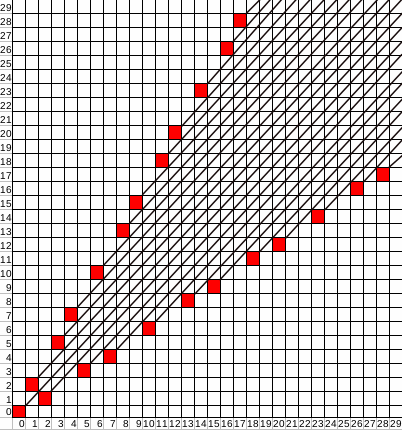
\includegraphics[width=0.8\textwidth]{../src/statistics/picture/p_positions_a=1.png}
			\end{minipage}
		\end{center}
	\end{frame}
	
	\begin{frame}{Рекурзивна стратегија}
		\begin{tcolorbox}[title=Дефиниција оператора $ \mex $]
			$\mex(A)$ означава најмањи природни број који није у скупу $ A $, тј. $ \mex(\emptyset)=0 $ и
			$ \mex(A)=\min\{i | i\notin A\} $.
		\end{tcolorbox}
	
	    \begin{tcolorbox}[title=Рекурзивна карактеризација изгубљених позиција]
	    	Све изгубљене позиције $ (A_{n}, B_{n}) $ могу се изразити на следећи начин:
	    	\begin{eqnarray*}
		    	&A_{n} = &\mex \{ A_{i}, B_{i} : i < n \}\\
		    	&B_{n} = &A_{n} + an
	    	\end{eqnarray*}
	   	\end{tcolorbox}
	\end{frame}

	\begin{frame}{Рекурзивна стратегија}
		\examplebox{За $ a \equal 1 $ неке изгубљене позиције су:}{
		\begin{table}[h!]
			\begin{center}
				\begin{tabular}{  c | c | c }
					{\textbf{n}} &  {\textbf{A}} &  {\textbf{B}} \\
					\hline
					0 & 0 & 0 \\
					1 & 1 & 1 + 1$ \cdot $1 = 2 \\
					2 & 3 & 3 + 1$ \cdot $2 = 5 \\
					3 & 4 & 4 + 1$ \cdot $3 = 7 
				\end{tabular}
			\end{center}
		\end{table}}
		\examplebox{За $ a \equal 2 $ неке изгубљене позиције су:}{
			\begin{table}[h!]
				\begin{center}
					\begin{tabular}{  c | c | c }
						{\textbf{n}} &  {\textbf{A}} &  {\textbf{B}} \\
						\hline
						0 & 0 & 0 \\
						1 & 1 & 1 + 2$ \cdot $1 = 3\\
						2 & 2 & 2 + 2$ \cdot $2 = 6\\
						3 & 4 & 4 + 2$ \cdot $3 = 10
					\end{tabular}
				\end{center}
		\end{table}}
	\end{frame}

	\begin{frame}{Алгебарска стратегија}
		\begin{tcolorbox}[title=Алгебарска карактеризација изгубљених позиција]
			Све изгубљене позиције $ (A_{n}, B_{n}) $ могу се изразити на следећи начин $ A_{n} = \lfloor \alpha \cdot n \rfloor, B_{n} = \lfloor \beta \cdot n \rfloor $, где је:
			\begin{eqnarray*}
				&\alpha = &\frac{2 - a + \sqrt{a^2 + 4}}{2} \label{def:alpha}\\  
				&\beta = &\alpha + a \label{def:beta},
			\end{eqnarray*}
	    	овде су $ \alpha $ и $ \beta $ ирационални за свако $ a > 0 $
		\end{tcolorbox}
	\end{frame}
	
	\begin{frame}{Алгебарска стратегија}
		\examplebox{За $ a \equal 2 $ онда је $ \alpha \equal \sqrt{3} $ и $ \beta \equal \sqrt{3} + 2 $ и неке изгубљене позиције су:}{
			\begin{table}[h!]
				\begin{center}
					\begin{tabular}{  c | c | c }
						{\textbf{n}} &  {\textbf{A}} &  {\textbf{B}} \\
						\hline
						0 & 0 & 0 \\
						1 & $ \lfloor \sqrt{3} \cdot 1 \rfloor = 1 $ & $ \lfloor (\sqrt{3} + 2) \cdot 1 = 3 \rfloor $\\
						2 & $ \lfloor \sqrt{3} \cdot 2 \rfloor = 2 $ & $ \lfloor (\sqrt{3} + 2) \cdot 2 = 6 \rfloor $\\
						3 & $ \lfloor \sqrt{3} \cdot 3 \rfloor = 4 $ & $ \lfloor (\sqrt{3} + 2) \cdot 3 = 10 \rfloor $\\
						4 & $ \lfloor \sqrt{3} \cdot 4 \rfloor = 5 $ & $ \lfloor (\sqrt{3} + 2) \cdot 4 = 13 \rfloor $\\
						5 & $ \lfloor \sqrt{3} \cdot 5 \rfloor = 7 $ & $ \lfloor (\sqrt{3} + 2) \cdot 5 = 17 \rfloor $
					\end{tabular}
				\end{center}
		\end{table}}
	\end{frame}
%	\begin{frame}{Рекурзивна и алгебарска карактеризација изгубљених позиција}
%		\begin{itemize}
%			\item Ако је $ x = B_{n} $ онда се из позиције $ (x = B_{n}, y) $ може једним потезом (скидањем жетона са гомиле на којој је $ y $ жетона) прећи у изгубљену позицију $ (A_{n}, B_{n}) $ 
%			\item Ако је $ x = A_{n} $ и $ y > B_{n} $, онда се смањивањем $ y $ може доћи у позицију $ (A_{n}, B_{n}) $. У противном, ако је 
%			$ A_{n} \leq y < B_{n} $ онда се смањивањем $ x $ и $ y $ може прећи у позицију $ (A_{m}, B_{m}) $, где је $ m = \lfloor \frac{d}{a} \rfloor $ и $ d = y - x $
%		\end{itemize}
%	\end{frame}
	
	\begin{frame}{Рекурзивна и алгебарска карактеризација изгубљених позиција}
		Нека је $ a = 2 $ и тренутна позиција $ (x, y) $ је:
		\begin{itemize}
			\item $ (17, 29) $, како је $ B_{5} = 17 $, то се из позиције $ (17, 29) $ уклањајући $ 22 $ жетона прелази у позицију $ (A_{5}, B_{5}) = (7, 17) $. 
			\item $ (11, 29) $, како је $ A_{8} = 11 $ и $ 29 > B_{8} = 27 $, то се из позиције $ (11, 29) $ уклањајући $ 2 $ жетона прелази у позицију $ (A_{8}, B_{8}) = (11, 27) $.
			\item $ (11, 25) $, како је $ A_{8} = 11 $ и $ 25 < B_{8} = 27 $, то се из позиције $ (11, 25) $ уклањајући по $ 2 $ жетона са обе гомиле прелази у позицију $ (A_{7}, B_{7}) = (9, 23) $.
		\end{itemize}
	\end{frame}
	
	
	\begin{frame}{Аритметичка стратегија}
		\begin{tcolorbox}
			[title=Нека је $ \leftbracket a_{0}\comma a_{1}\comma a_{2}\comma \ldots \rightbracket $ верижни развој броја $ \alpha $ и за низове $ p_{n} $ и $ q_{n} $ (бројилаца и именилаца конвергената) важи следећа рекурентна релација:]
				$ p_{-1} = 1,\ p_{0} = a_{0},\ p_{n} = a_{n}p_{n-1} + p_{n-2},\ (n \geq 1 )\\
				q_{-1} = 0,\ q_{0} = 1,\ q_{n} = a_{n}q_{n-1} + q_{n-2},\ (n \geq 1 ) $
		\end{tcolorbox}
	
		\examplebox{Нека је верижни развој броја $ \alpha \equal \leftbracket 1\comma 2\comma 2 \ldots \rightbracket \equal 1 + \frac{1}{2 + \frac{1}{2 + \ldots}} $ чији су конвергенти:}
		{$ 	C_{0} = 1 = \frac{p_{0}}{q_{0}},\\ 
			C_{1} = [1, 2] = 1 + \frac{1}{2} = \frac{3}{2} = \frac{p_{1}}{q_{1}},\\ 
			C_{3} = [1, 2, 2] = 1 + \frac{1}{2 + \frac{1}{2}} = \frac{7}{5} = \frac{p_{3}}{q_{3}},\\ \ldots $}	
	\end{frame}
	
	\begin{frame}{Аритметичка стратегија}
		\begin{tcolorbox}[title=Репрезентација $ R $ је:]
			$ R = (d_{m}, d_{m-1}, \ldots , d_{1}, d_{0}), \ 0 \leq d_{i} \leq a_{i+1} $
		\end{tcolorbox}
		\begin{tcolorbox}[title=$ p $-репрезентација $ R_{p} $ броја $ k $ је:]
			$ R_{p}(k) = (d_{m}, d_{m-1}, \ldots , d_{1}, d_{0}) $
		\end{tcolorbox}
		\begin{tcolorbox}[title=$ q $-репрезентација $ R_{q} $ броја $ k $ је:]
			$ R_{q}(k) = (d_{m}, d_{m-1}, \ldots , d_{1}, d_{0}) $
		\end{tcolorbox}
	\end{frame}
	
	\begin{frame}{Приказ првих $ 15 $ бројева записаних у $ p $ и $ q $ систему, за $ a_{i} = 2 $, $ i \geq 1 $}
		\begin{table}[h!]
			\begin{center}
				\begin{tabular}{ | c | c | c | c | c  c | c | c | c | c | c |}
					\hline
					{$ \mathbf{q_{3}} $} &  {$ \mathbf{q_{2}} $} &  {$ \mathbf{q_{1}} $} &  {$ \mathbf{q_{0}} $} & & &  {$ \mathbf{p_{3}} $} &  {$ \mathbf{p_{2}} $} &  {$ \mathbf{p_{1}} $} &  {$ \mathbf{p_{0}} $} &\\
					12 & 5 & 2 & 1 & & & 17 & 7 & 3 & 1 &  {$ \mathbf{n} $}\\
					\hline
					&  &  & 1 & & &  &  &  & 1 & {$ \mathbf{1} $}\\
					&  & 1 & 0 & & &  &  &  & 2 & {$ \mathbf{2} $}\\
					&  & 1 & 1 & & &  &  & 1 & 0 &  {$ \mathbf{3} $}\\
					&  & 2 & 0 & & &  &  & 1 & 1 &  {$ \mathbf{4} $}\\
					& 1 & 0 & 0 & & &  &  & 1 & 2 &  {$ \mathbf{5} $}\\
					& 1 & 0 & 1 & & &  &  & 2 & 0 &  {$ \mathbf{6} $}\\
					& 1 & 1 & 0 & & &  & 1 & 0 & 0 &  {$ \mathbf{7} $}\\
					& 1 & 1 & 1 & & &  & 1 & 0 & 1 &  {$ \mathbf{8} $}\\
					& 1 & 2 & 0 & & &  & 1 & 0 & 2 &  {$ \mathbf{9} $}\\
					& 2 & 0 & 0 & & &  & 1 & 1 & 0 &  {$ \mathbf{10} $}\\
					& 2 & 0 & 1 & & &  & 1 & 1 & 1 &  {$ \mathbf{11} $}\\
					1 & 0 & 0 & 0 & & & & 1 & 1 & 2 &  {$ \mathbf{12} $}\\
					1 & 0 & 0 & 1 & & & & 1 & 2 & 0 &  {$ \mathbf{13} $}\\
					1 & 0 & 1 & 0 & & & & 2 & 0 & 0 &  {$ \mathbf{14} $}\\
					1 & 0 & 1 & 1 & & & & 2 & 0 & 1 &  {$ \mathbf{15} $}\\
					\hline 
				\end{tabular}
			\end{center}
		\end{table}
	\end{frame}
	
	\begin{frame}{Аритметичка стратегија}
		\begin{tcolorbox}[title=Леви померај репрезентације $ R $ је:]
			$ R^{'} = (d_{m}, d_{m-1}, \ldots , d_{1}, d_{0}, 0) $
		\end{tcolorbox}
		\begin{tcolorbox}[title=Десни померај репрезентације $ R $ је:]
			$ R^{''} = (d_{m}, d_{m-1}, \ldots , d_{1}) $
		\end{tcolorbox}
		\begin{tcolorbox}[title=Веза $ p $-интерпретације $ I_{p} $ и $ q $-репрезентације $ R_{q} $ је:]
			$ I_{p}(R_{q}(k)) = I_{p}(d_{m}, d_{m-1}, \ldots, d_{0}) $
		\end{tcolorbox}
	\end{frame}
	
%	\begin{frame}{Аритметичка карактеризација изгубљених позиција}
%		
%		Уколико је текућа позиција $ (x, y), 0 < x \leq y $, прво се рачуна $ R_{p}(x) $ и проверава се да ли се завршава парним или непарним бројем нула.
%		subsection
%		\begin{enumerate}
%			\item \label{item:neparne_nule} Уколико се $ R_{p}(x) $ завршава непарним бројем нула, онда је $ x = B_{n} $, тако да је победнички потез $ (x, y) \rightarrow (I_{p}(R^{''}_{p}(x)), x) $.
%			\item \label{item:parne_nule} Уколико се $ R_{p}(x) $ завршава парним бројем нула, онда је $ x = A_{n} $. Ако је $ y > I_{p}(R^{'}_{p}(x)) $ победнички потез је $ (x, y) \rightarrow (x, I_{p}(R^{'}_{p}(x)) $. У противном, ако је $ y < I_{p}(R^{'}_{p}(x) $, рачунамо $ d = y - x, m = \lfloor \frac{d}{a} \rfloor $. Уколико се $ R_{q}(m) $ завршава парним бројем нула, онда је $ A_{m} = I_{p}(R_{q}(m)) $; у противном je $ A_{m} = I_{p}(R_{q}(m)) + 1 $.
%			У оба случаја победнички потез је $ (x, y) \rightarrow (A_{m}, A_{m} + ma) $.
%		\end{enumerate}		
%	\end{frame}
	
	
		\begin{frame}{Аритметичка карактеризација изгубљених позиција}
		
		Нека је $ a = 2 $ и тренутна позиција $ (x, y) $ je:
		\begin{itemize}
			\item $ (17,29) $, како се $ R_{p}(17) = (1, 0, 0, 0)$ завршава непарним бројем нула, онда је $ B_{5} = 17 $ и $ I_{p}(R^{''}_{p}(17) = I_{p}(1, 0, 0) = 7 $ па је победнички потез $ (7, 17) $.
			\item $ (11, 29) $, како се $ R_{p}(11) = (1, 1, 1) $ завршава парним бројем нула, онда је $ A_{8} = 11 $ и $ I_{p}(R^{'}_{p}(11)) = I_{p}(1, 1, 1, 0) = 27 $ па пошто је $ 29 > 27 $ победнички потез је $ (11, 27) $.
			\item $ (11, 23) $, како се $ R_{p}(11) = (1, 1, 1) $ завршава парним бројем нула, онда је $ A_{8} = 11 $ и $ I_{p}(R^{'}_{p}(11)) = I_{p}(1, 1, 1, 0) = 27 $, па пошто је $ 23 < 27 $ рачуна се $ R_{q}(\lfloor \frac{y - x}{a} \rfloor) = R_{q}(6) = (1, 0, 1) $ и $ I_{p}(R_{q}(6)) = 8 $ па је победники потез $ (8, 20) $.
			\item $ (11, 25) $, како се $ R_{p}(11) = (1, 1, 1) $ завршава парним бројем нула, онда је $ A_{8} = 11 $ и $ I_{p}(R^{'}_{p}(11)) = I_{p}(1, 1, 1, 0) = 27 $, па пошто је $ 25 < 27 $ рачуна се $ R_{q}(\lfloor \frac{y - x}{a} \rfloor) = R_{q}(7) = (1, 1, 0) $ и $ I_{p}(R_{q}(7)) = 10 $ па је победники потез $ (9, 23) $.
		\end{itemize}		
	\end{frame}
	
\section{Евалуација решења}

%\begin{frame}{Имплементација и евалуација}
%	
%	\begin{figure}
%		\centering
%		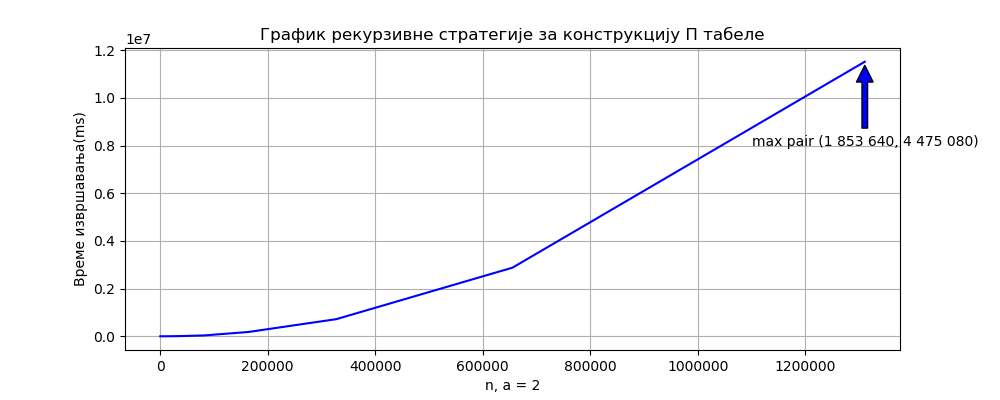
\includegraphics[width=0.8\textwidth]{../src/statistics/picture/recursive.png}
%		\caption{График рекурзивне стратегије за конструкцију табеле изгубљених позиција
%		за $ n $ до $ 41943040 $}
%	\end{figure}
%	
%\end{frame}
%
%\begin{frame}{Имплементација и евалуација}
%	
%	\begin{figure}
%		\centering
%		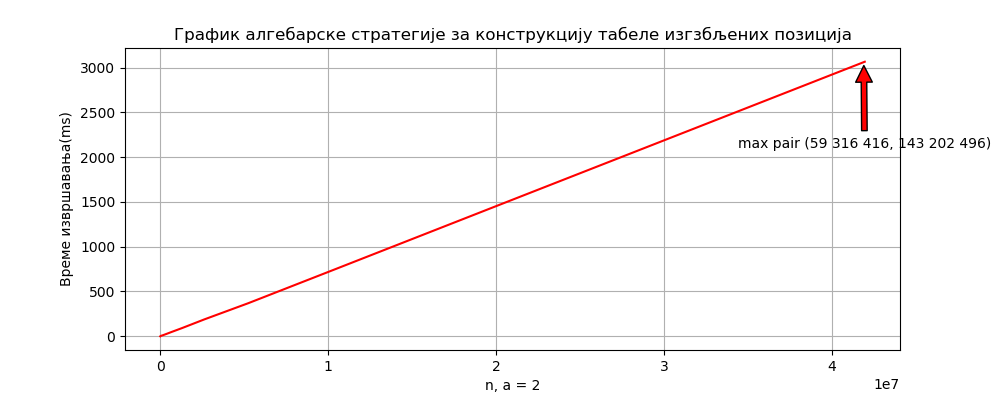
\includegraphics[width=0.8\textwidth]{../src/statistics/picture/algebraic.png}
%		\caption{График алгебарске стратегије за конструкцију табеле изгубљених позиција за $ n $ до $ 41943040 $}
%	\end{figure}
%	
%\end{frame}
%
%\begin{frame}{Имплементација и евалуација}
%	
%	\begin{figure}
%		\centering
%		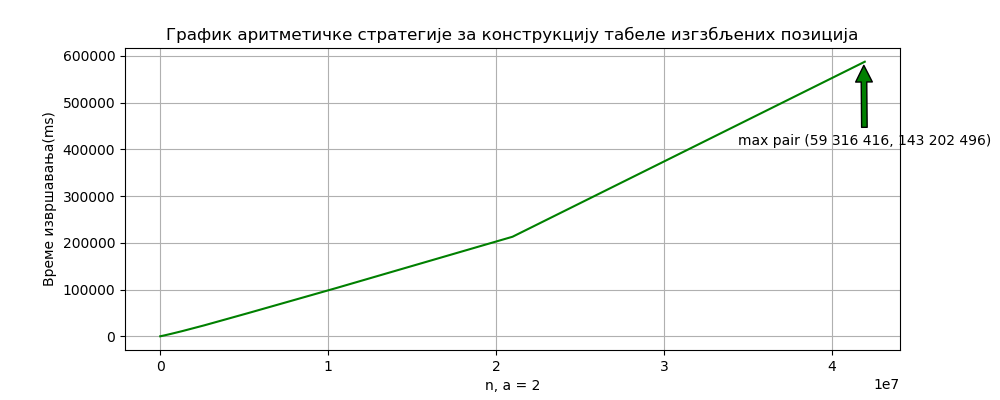
\includegraphics[width=0.8\textwidth]{../src/statistics/picture/arithmetic.png}
%		\caption{График аритметике стратегије за конструкцију табеле изгубљених позиција за $ n = 41943040 $}
%	\end{figure}
%	
%\end{frame}

\begin{frame}{Евалуација решења}
	\begin{figure}[H]
		\begin{center}
			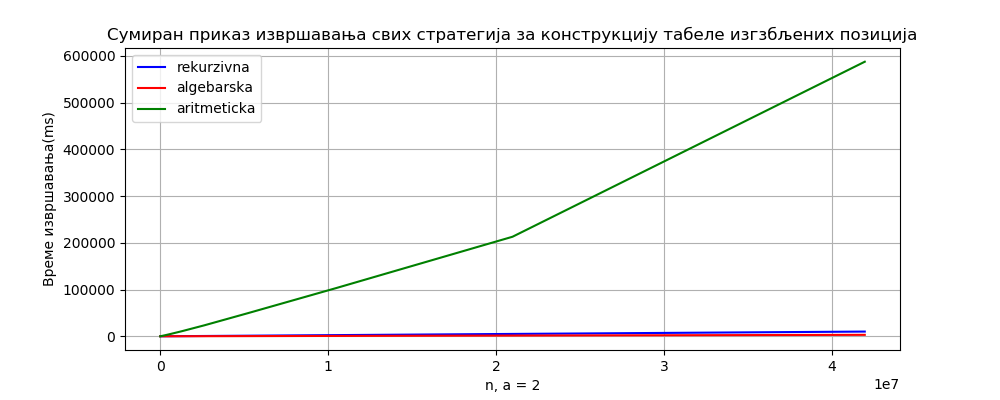
\includegraphics[width=\textwidth]{../src/statistics/picture/all.png}
		\end{center}
		\caption*{Сумирани приказ извршавања свих стратегија за конструкцију табеле изгубљених позиција}
	\end{figure}
\end{frame}

\begin{frame}{Евалуација решења}	
	\begin{figure}[H]
		\begin{center}
			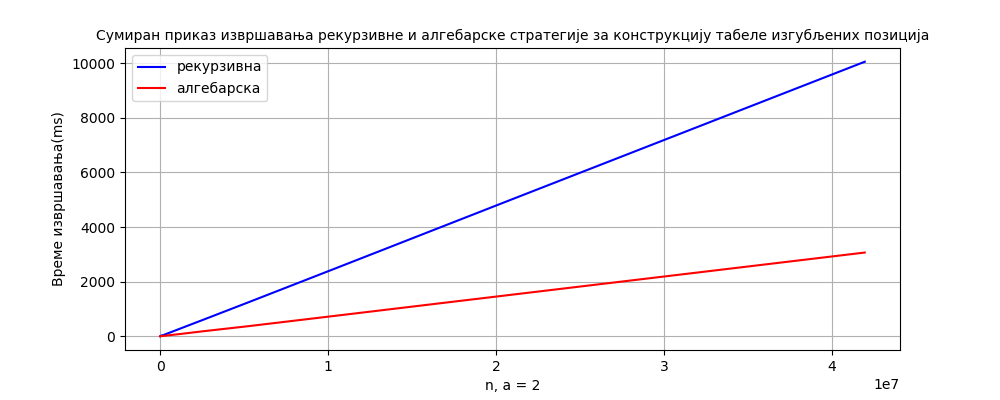
\includegraphics[width=\textwidth]{../src/statistics/picture/algebraicVSrecursive.png}
		\end{center}
		\caption*{Сумирани приказ извршавања рекурзивне и алгебарске стратегије за конструкцију табеле изгубљених позиција}
	\end{figure}
\end{frame}

\begin{frame}{Крај}
	\begin{center}
		Хвала на пажњи!\\
		Питања?
	\end{center}
\end{frame}

\end{document}